\section{Results}

\subsection{Idea Forest}

Hierarchical clustering yielded an idea forest composed of 3007 instances, 1213 unique ideas, 335 category trees, and 129 non-singleton category trees (Table~\ref{tab:idea_forest}). The number of nodes within a category tree ranged from 1 to 66, with the distribution of values roughly following a Poisson distribution. The number of instances per node (i.e., the number of equivalent idea instances) also roughly follows a Poisson distribution, with the number of instances ranging from 1 to 63.
\begin{table}
	\begin{tabular}[h!]{r | l l l l l l l}
	\textbf{number requested} & 5 & 10 & 20 & 50 \\ \hline \hline
	HITs & 57 & 47 & 23 & 10\\
	instances & 293 & 471 & 453 & 500 \\
	ideas & 171 & 249 & 278 & 341 \\
	category trees & 72 & 79 & 93 & 114 \\
	non-singleton trees & 28 & 34 & 40 & 48 \\ \hline \hline
	\textbf{number requested} & 75 & 100 & all \\ \hline \hline
    HITs & 10 & 10 & 146\\
	instances & 634 & 855 & 3007\\
	ideas & 443 & 177 &1212\\
	category trees & 172 & 177 &321\\
	non-singleton trees & 49 & 61 &92\\ 
	\end{tabular}
    \caption{Result counts between conditions}
    \label{tab:idea_forest}
\end{table}

% are also roughly poisson distributed (Table TAB). In keeping with the findings for height, trees found in the upper number conditions are smaller than trees found in the lower conditions. The precipitous drop in median tree size suggests that in the largest condition, participants are finding rare ideas with only a few variants and less than 14 instances.

% \begin{table}
% \begin{tabular}[h!]{r | l l l l l l l}
% 	\textbf{number condition} & 5 & 10 & 20 & 50 & 75 & 100 & all \\ \hline \hline
% 	number of nodes& \\ \hline
%     median &5&5&4&3&2&2&2 \\
% 	first quartile &2&2&1&1&1&1&1 \\
% 	third quartile &17&17&14&10&5&5&5 \\
% 	number of instances& \\ \hline
% 	median &14&14&12&10&4&4&4 \\
%     first quartile &4&4&4&2&1&1&1 \\
% 	third quartile &47&45&30&23&13&13&13 \\
% 	\end{tabular}
% 	\caption{Number of ideas and instances in trees}
% \end{table}

% \begin{figure}[h!]
%     \centering
%     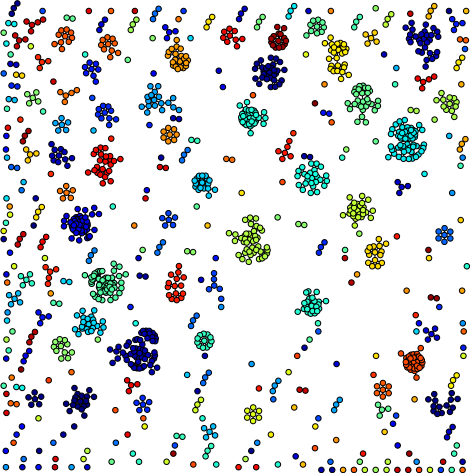
\includegraphics[width=0.9\columnwidth]{idea_forest}
%     \caption{Idea Forest}
% \end{figure}

% The height of category trees follows a roughly Poisson distribution, with the maximum tree height observed at 5. Summary statistics across condition are in table TAB. The third quartile drops as the number condition increases. While the upper conditions still discover categories trees with heights as great as 5, they generate many more "short" trees. This suggests that the ideas generated in the upper conditions are less common.

% \begin{table}
% 	\begin{tabular}[h!]{r | l l l l l l l}
% 	\textbf{number condition} & 5 & 10 & 20 & 50 & 75 & 100 & all \\ \hline \hline
% 	median & 2 & 2 & 2 & 2 & 2 & 2 & 2\\
% 	first quartile & 2 & 2  & 1 & 1 & 1 & 1 & 1\\
% 	third quartile & 3 & 3 &3 &3 &2 &2 & 2\\
% 	\end{tabular}
% 	\caption{Category tree height}
% \end{table}

\subsection{Rates of Idea and Category Production}
Using the fully clustered data set, we can model the rate at which unique ideas and unique categories of ideas are produced, testing hypothesis 1 (i.e., the notion that rates of unique ideas and categories of ideas are non-linear over time).

Figure~\ref{fig:cumulative_ideas} shows the cumulative count of unique ideas per condition, as a function of the number of instances gathered in the experiment. The plots for each condition were obtained by considering each response instance in the order in which it was received, with its uniqueness assessed relative to all response instances received before it. For reference, an ideal ``1:1'' idea generation line is also plotted.

We model this quantity using the following exponential model:
\[n_{ideas} = y_{scale} * x^{rate}\]
where $n_{ideas}$ represents the number of unique ideas, $y_{scale}$ serves to scale the model, $x$ is the response number, and $rate$ models the rate of novel ideas. Importantly, this simplified model does not model either the condition or the effects of workers. In our analysis of the data, we found that individual workers introduced considerable variation, preventing us from separating the effects of the condition from the worker. Accordingly, we only consider this simplified model.

Fitting this model with Stan, we obtain a $y_{scale}$ value of 1.49 (HDI 1.44-1.55) and a $rate$ value of 0.87 (HDI 0.86-0.88). Because $rate$'s HDI does not include 1, we find support for hypothesis 1: the number of unique ideas is non-linear as a function of the number of responses received. The fitted model is shown as the ``Best Fit'' line in Figure~\ref{fig:cumulative_ideas}.

\begin{figure}[h!]
    \centering
    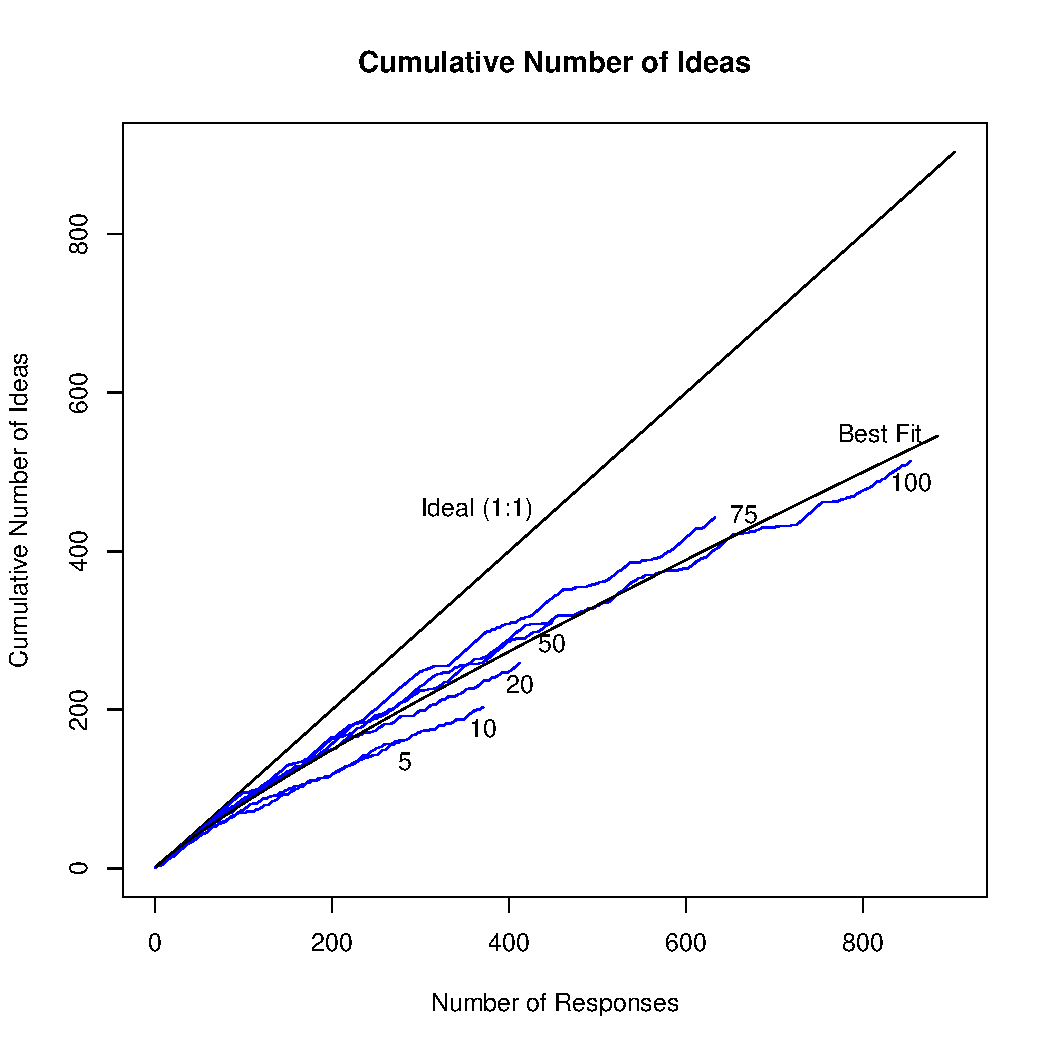
\includegraphics[width=0.9\columnwidth]{cumulative_ideas}
    \caption{Cumulative number of novel ideas}
    \label{fig:cumulative_ideas}
\end{figure}

\begin{figure}[h!]
    \centering
    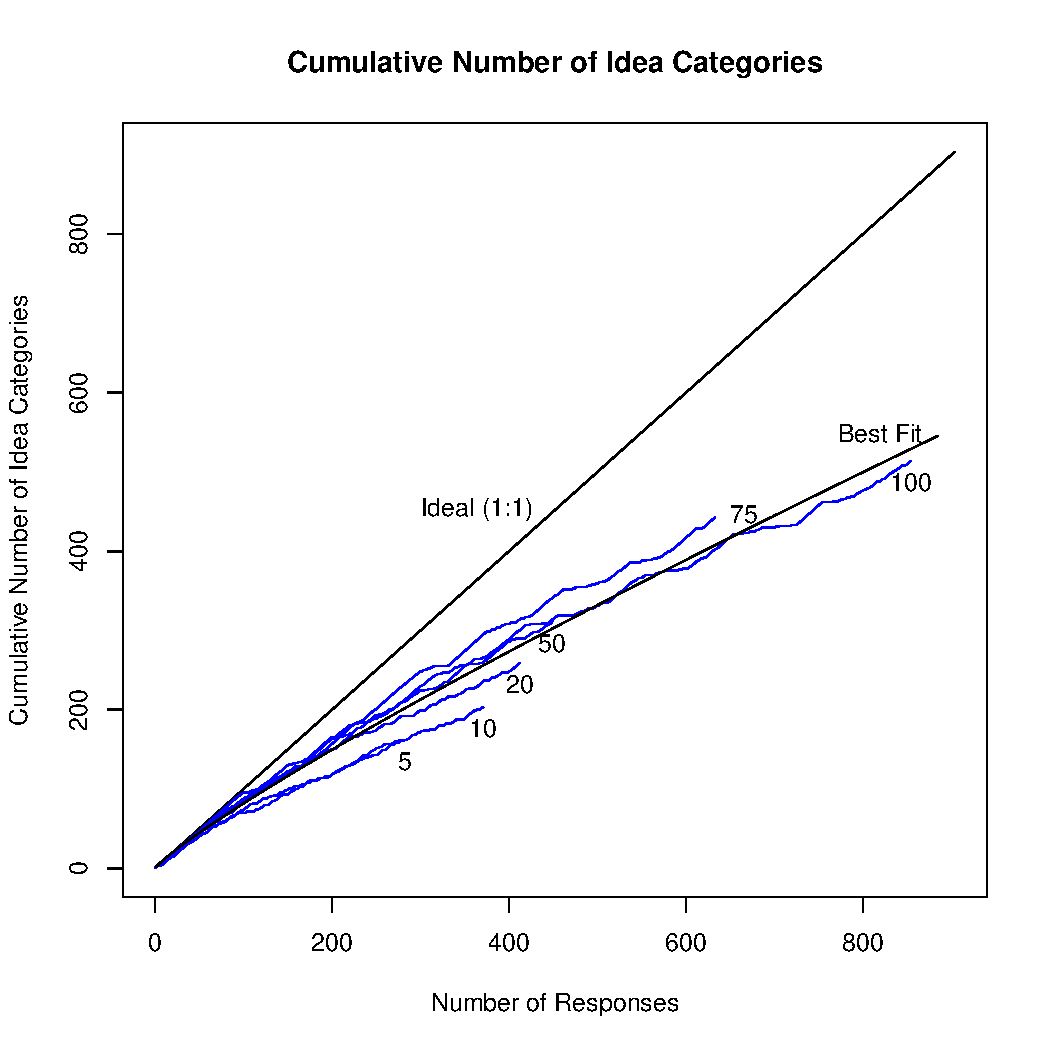
\includegraphics[width=0.9\columnwidth]{cumulative_categories}
    \caption{Cumulative number of novel idea categories}
    \label{fig:cumulative_categories}
\end{figure}

% \begin{figure}[h!]
%     \centering
%     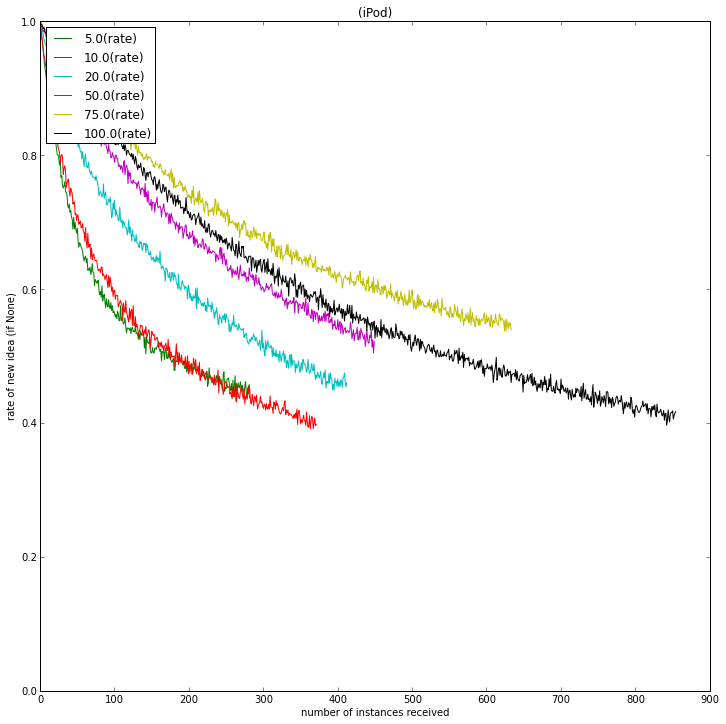
\includegraphics[width=0.7\columnwidth]{rate_new_idea_over_time}
%     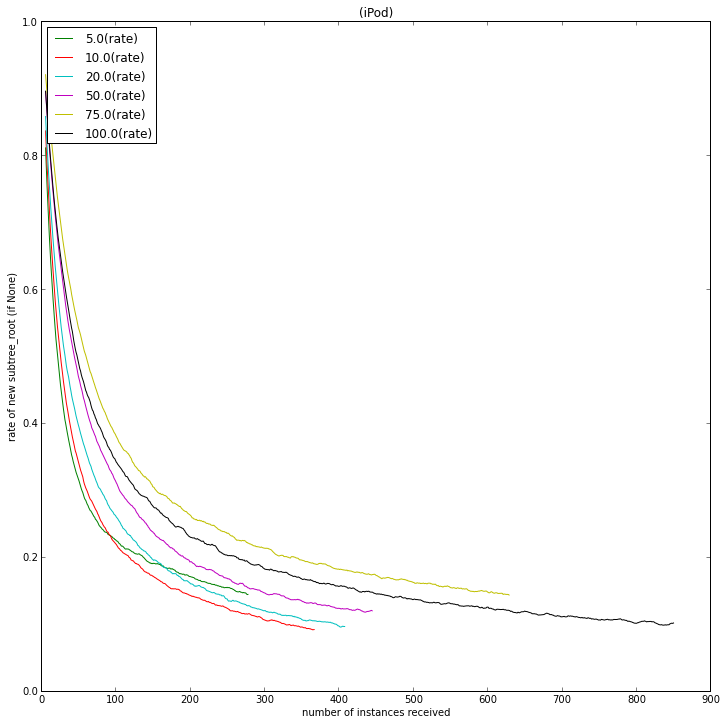
\includegraphics[width=0.7\columnwidth]{rate_new_category_over_time}
%     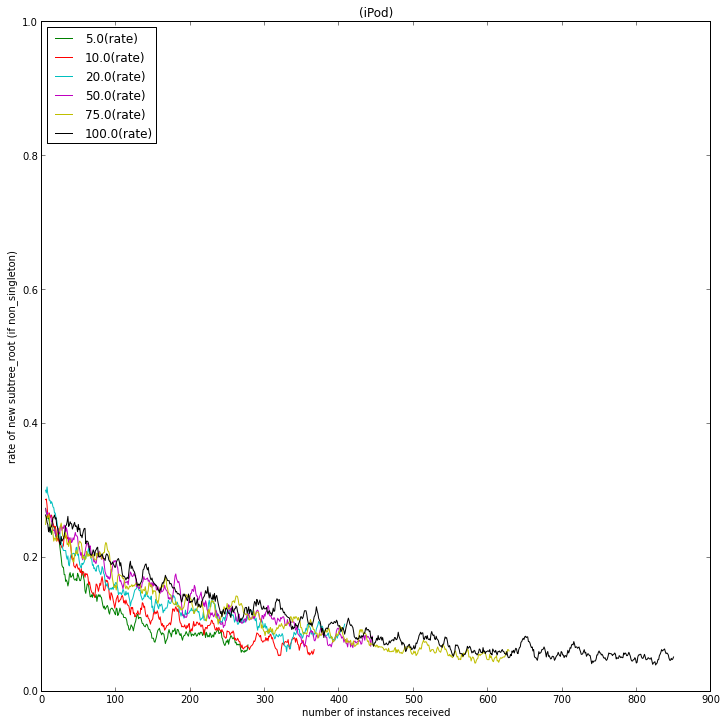
\includegraphics[width=0.7\columnwidth]{rate_new_ns_category_over_time}
%     \caption{Rate of idea generation}
% \end{figure}

We use an identical model for modeling the rate at which new idea categories are introduced over time. Figure~\ref{fig:cumulative_categories} shows the data and fitted model for the cumulative number of novel categories over time. For this model, we obtain a $y_{scale}$ value of 2.1 (HDI 2.0-2.2), with a $rate$ of 0.67 (HDI 0.66-0.67). Again, we find very clear support that the rate of novel categories is non-linear as a function of the number of responses received.

The visibly lower rate of growth for novel categories growth suggests workers are more likely to produce new ideas within existing categories, rather than create both novel ideas that also represent novel categories. We more closely examine characteristics of individuals' brainstorming runs next.

%Given the observed differences in production of new ideas and idea categories, it is worthwhile to better understand \emph{why} these differences exist. 

%The third panel, which shows non-singleton categories over time, tells a distinctly different story from the others. While in the idea and category plots, the height-ordering of rates of generation between categories remains generally identical, there is a point of intersection and reversal in the non-singleton category plot at around the 30 instances point. Before this point, the lower conditions actually generate new categories at a \emph{faster} rate.

\subsection{Characteristics of an Idea Within a Run}

\subsubsection{Most Popular Ideas}
Our data suggest that individuals typically produce ideas from a common set of idea categories early in the brainstorming process, then diverge and produce more original ideas. This phenomenon can be observed by examining the o-scores of ideas and idea categories.

Figures~\ref{fig:idea_oscore_order} and \ref{fig:cat_oscore_order} show the o-scores for response instances and idea categories, within a sliding window of size 10. Each point represents the mean o-score within that sliding window, with standard error bars provided for each point.


%As our measure of originality, we use \emph{o-score}, introduced by Jansson and Smith \cite{jansson_design_1991}. An idea's o-score is $1 - p(idea)$, where $p(idea) = (number of instances of that idea)/(number of instances total)$. The o-score for category trees is similarly calculated. We will occasionally refer to the \emph{category o-score} of an idea. This simply refers to the o-score of the category tree to which that idea belongs.

% We measure differences in originality between conditions by examining the idea o-score and category o-score. The distributions of these scores are summarized in Figure FIG. The left panel compares idea o-score and the right compares category o-score.

%. Beyond the inflection point, the category pool is saturated with these low-hanging fruit, and only brainstormers tasked with generating more ideas will find the smaller category. This is a more nuanced view of the tree node/instance quartiles in Section SEC; condition 5 brainstormers cover the spectrum of category sizes while condition 100 brainstormers pull from the smaller category trees in the forest.



% The final measure, \emph{look-back equality}, is non-symmetrical and has meaning only in the context of a single brainstorming run. An instance \emph{a} is look-back equal to an \emph{earlier} instance \emph{b} if \emph{b} is in either \emph{a}'s idea node or any of \emph{a}'s parents, siblings, or children. This definition specifically identifies when a later instance in a run can be considered to have been influenced by earlier instance.



% \begin{figure}[h!]
%     \centering
%     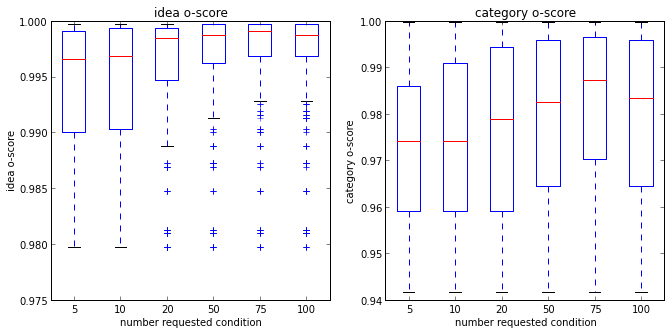
\includegraphics[width=0.9\columnwidth]{oscores_conditions}
% \end{figure}

% The more ideas requested, the more original the ideas produced. As suggested by the instance quartile range in section SEC, higher number conditions produce idea in trees with fewer instances, thus the high category o-score. We also see that these conditions produce \emph{ideas} with fewer instances.

% As the originality rises, however, so does the number of outliers. To understand this phenomenon, we need to more closely observe the distribution of originality scores between not just conditions, but ordinal position in a brianstorming run.

% Figure FIG provides this visualization. The upper panel gives the mean idea o-score as a function of ordinal position in all 100 condition brainstorming runs. The o-score for each ordinal position is the mean of all idea o-scores for that ordinal position in a run. Following this, the plot is further smoothed by making each point the mean of a sliding window of size 10 around its ordinal position. The bottom panel is a similar plot for category-oscore. To aid in interpretation, the first, second and third quartiles are also represented on the plot. The error bars are standard error.

% \begin{figure}[h]
%     \centering
%     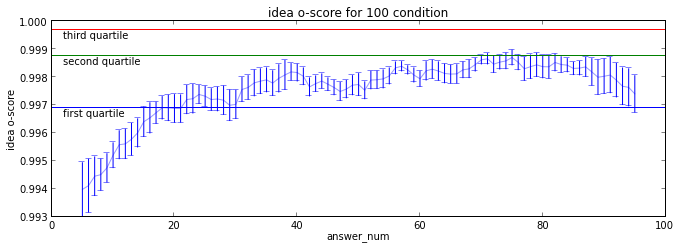
\includegraphics[width=0.9\columnwidth]{idea_oscore_order_100}
%     \caption{Idea o-score as a function of order (100 condition)}
%     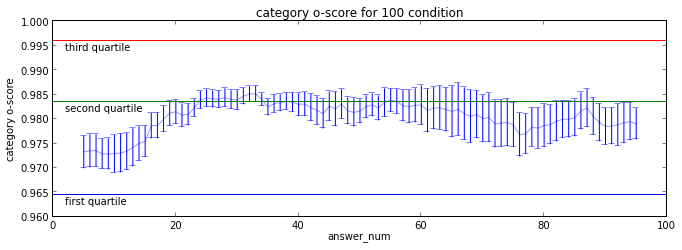
\includegraphics[width=0.9\columnwidth]{cat_oscore_order_100}
%     \caption{Category o-score as a function of order (100 condition)}
% \end{figure}

% The only part of the originality score that falls outside the first and third quartiles is the beginning of the run. Participants in the higher numbered conditions generate more original ideas overall, but not until they have exceeded some threshold of common ideas. Figure FIG replicates figure FIG but across all conditions, and the same pattern of originality growth until an originality peak - around 20 ideas - is reached. Note that because of the additional HITs, there are far more examples of early-order ideas in the 5, 10 and 20 conditions than in the 50, 75, or 100, so this pattern is present without any dominating affect by the upper conditions.

\begin{figure}[h]
    \centering
    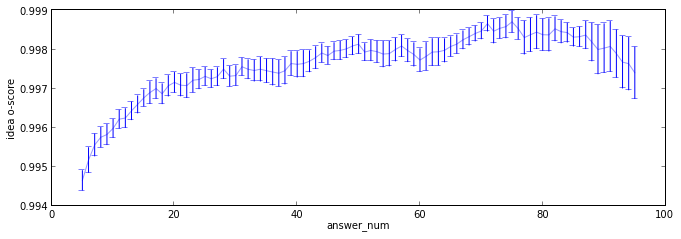
\includegraphics[width=0.9\columnwidth]{idea_oscore_order}
    \caption{Idea o-score as a function of response number, all conditions}
    \label{fig:idea_oscore_order}
    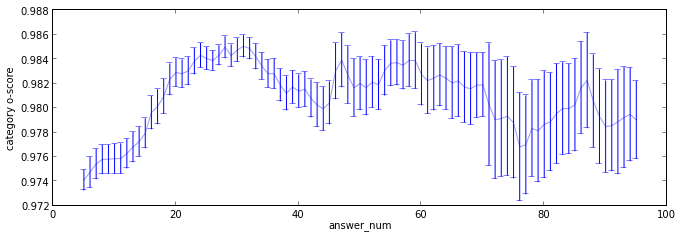
\includegraphics[width=0.9\columnwidth]{cat_oscore_order}
    \caption{Category o-score as a function of response number, all conditions}
    \label{fig:cat_oscore_order}
\end{figure}

In both cases, we observe a steady increase in o-scores for the first 20-30 responses. After these first 20-30 responses, the o-scores plateau, with no clear discernible pattern for either ideas or idea categories.

These graphs lend support for hypothesis 2, the notion that there is a set of general, common ideas that make up the first several responses of every crowd brainstorming session, regardless of condition.

To more explicitly confirm this hypothesis, we extracted the top 5\% most common ideas (66 in total). If individuals are more likely to initially generate the same set of ideas, the top 5\% of the ideas should be more likely to appear in the first five instances of a run than they are to appear in any of the following instances. We introduce two Bernoulli random variables to model this. The first, defined by parameter $\theta_f$ represents the probability that a response instance is in the top 5\% most common ideas, given it is found in the first five instances of a run (i.e., $P(\theta_f|top)$). The second, defined by parameter $\theta_l$, is the probability that an instance is in the top \% given it is one of the \emph{last} ($\textgreater5$) instances in a run (i.e., $P(\theta_l|\overline{top})$).

We fit these parameters using data from all runs that have more than 10 responses. We chose this constraint so that no run could contribute evidence to $\theta_f$ without also contributing to $\theta_l$. Using an uninformative beta prior, the resulting parameters are $\theta_f = 0.56$ (95\% HDI 0.52-0.61) and $\theta_l = 0.32$ (95\% HDI 0.30-0.34). This difference is significant, supporting the hypothesis that common ideas are over-represented in the early part of a brainstorming run.


%This is explained by the relationship between common ideas and common categories. We expect that unoriginal ideas belong to unoriginal categories, as a high instance count for an idea increases the instance count for its category tree. However, we cannot make the inverse assumption, that a high originality idea belongs to a high originality category. Once the common idea are exhausted, then, there is no relationship between idea originality and category originality.

\subsubsection{Originality}

The increase in o-score over time in Figures~\ref{fig:idea_oscore_order} and \ref{fig:cat_oscore_order} also supports hypothesis 3, the notion that ideas generated in the second half a brainstorming session have higher o-scores than those in the first half. We test a stronger guarantee of this hypothesis that is implied by our data: that ideas after the first 20 have higher o-scores than the first 20.

Partitioning the data into instances $\leq20$ and $\textgreater20$, we found that these distributions of o-scores are best modeled using beta distributions. Figures~\ref{fig:idea_oscore_hyp4} and \ref{fig:cat_oscore_hyp4} show the data and fitted models. Examining the HDIs of the resultant model parameters shows significant differences between the models, confirming hypothesis 3.

Collectively, these results provide a clear guideline for maximizing originality in brainstorming tasks on microtask marketplaces: it is more cost-effective to solicit $\textgreater20$ ideas from a smaller pool of participants than to ask for fewer ideas from more individuals.


%The $\alpha$ parameter is significantly different in both the idea and category o-score comparison. The mean idea o-score is 0.997 in the $\textgreater20$ versus 0.995 in the $\leq20$ condition. Similarly, the $\leq20$ condition is favourable in category o-score with a mean of 0.982 vs 0.975.


% \begin{table}
% 	\begin{tabular}[h!]{r | l l }
% 	    & $\alpha$ median & $\alpha$ 95\% HDI \\ \hline \hline
%         idea o-score (\textless=20) & 135.86 & 122.39-149.72 \\
%         idea o-score (\textgreater20) & 259.84 & 240.47-278.81 \\ \hline \hline
% 	    & $\beta$ median & $\beta$ 95\% HDI \\ \hline \hline
%         category o-score (\textless=20) & 1.16 & 1.08-1.25 \\
%         category o-score (\textgreater20) & 0.82 & 0.77-0.86 \\
% 	\end{tabular}
%     \caption{Hypothesis 4 Beta models}
%     \label{tab:hyp4}
% \end{table}

\begin{figure}[h]
    \centering
    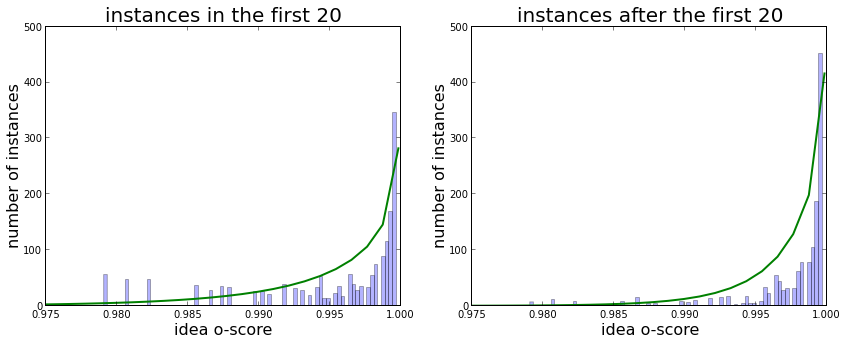
\includegraphics[width=0.9\columnwidth]{hyp4_ideas}
    \caption{Beta models for idea o-score}
    \label{fig:idea_oscore_hyp4}
    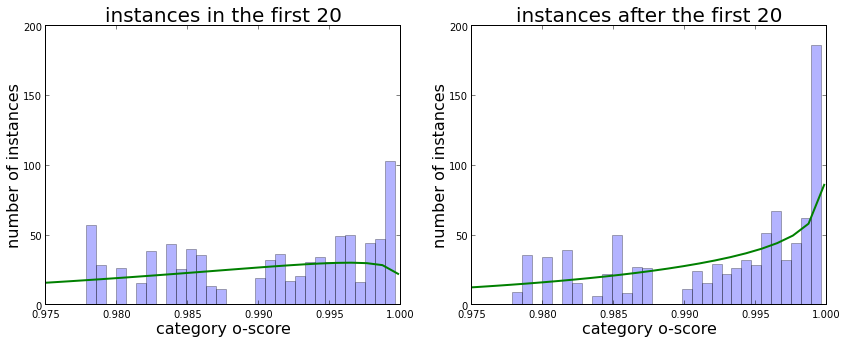
\includegraphics[width=0.9\columnwidth]{hyp4_cats}
    \caption{Beta models for category o-score}
    \label{fig:cat_oscore_hyp4}
\end{figure}






\subsection{Idea Generation Patterns}
Given the clear differences in idea characteristics as a function of response number, we now consider idea generation patterns observable from the data. In this section, we examine these patterns in the context of hypotheses 4 and 5, the hypotheses that draw upon the SIAM model of brainstorming. This model predicts individuals will generate ideas within ``images'' or categories of ideas (i.e., ``riff'' on an idea or concept) before switching to a new category.

In our clustered data, we can identify riffing by examining whether a response instance belongs to the same category tree as the previous instance. We can then derive a number of statistics from these data.

To contextualize this process, below is an excerpt of a particular participant's brainstorming run.

\begin{quote}
    \begin{enumerate}
        \item recycle
        \item take apart and refurbish
        \item scrap it for any precious metals inside (some have gold contacts)
    \end{enumerate}
\end{quote}

The participant first touches on the general idea of recycling, then becomes more specific by reducing the scope of recyling to specific parts. Finally, they limit the scope of parts to precious metals, particularly gold. At this point, the participant exhausts their working memory of the category and moves on.

Table~\ref{tab:riffing} provides a summary of riffing statistics observed in our data set. We find that the higher the number of instances requested, the more likely participants are to use old ideas as inspiration for new ideas. However, we observe that riff sequences are typically quite small in length, across conditions.

%An example of a single participant's riffed responses is given in Figure FIG. The second column is dark if the response instance is a permutation of any idea earlier in the run. The first column is dark if the instance is a \emph{source} instance, meaning it is the source for later permutations. Permutation chains can either be consecutive (as in this example), or separated with instances in between. The third column simply provides the text for that instance.

% \begin{figure}[h]
%     \centering
%     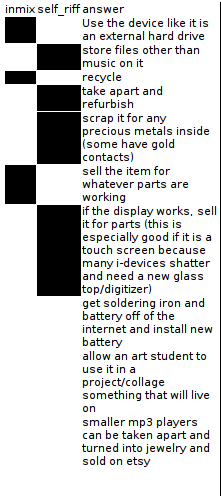
\includegraphics[width=0.5\columnwidth]{10_riff}
%     \caption{Example of riffing in a size 10 run}
% \end{figure}

%The participant hits on the categories of using the device's hard drive for storage, recycling the device or its materials, and selling the device.  within these categories, they generate 2-3 ideas each. This is a fairly typical example of riffing. In larger conditions, it is common for participants to reach further back and return to an idea multiple time. Table TAB provides a summary of riffing between conditions.

\begin{table}
\begin{tabular}[h!]{r | l l l l l l l}
    \hline \hline \textbf{condition} & 5 & 10 & 20  \\ \hline \hline
    \% riffs & 13.65 & 19.28 & 25.17  \\
    source instances & 10.58 & 12.92 & 15.01 \\
    riffs per source & 1.29 & 1.49 & 1.68 \\
    median length of consecutive chain & 2 & 2 & 2 \\
    median distance to previous in chain & 1 & 2 & 2 \\
    median distance to first in chain & 2 & 3 & 5 \\ \hline \hline
    \textbf{condition} & 50 & 75 & 100 \\ \hline \hline
    \% riffs & 39.6 & 32.81 & 42.81 \\
    source instances & 19 & 17.19 & 18.13\\
    riffs per source & 2.08 & 1.91 & 2.36\\
    median length of consecutive chain & 2 & 2 & 2\\
    median distance to previous in chain & 7 & 10 & 5\\
    median distance to first in chain & 16.5 & 18 & 26.5 \\
    \end{tabular}
    \caption{Riffing statistics by condition}
    \label{tab:riffing}
\end{table}


SIAM predict that individuals will generate ideas from an idea category until they exhaust that category, at which point they switch to another category (hypothesis 4). Furthermore, SIAM predicts that this category switching will be observable as taking more time to generate an idea in a new category than in the existing category (hypothesis 5). We examine each of these hypotheses in turn.

\subsubsection{Category changing}

To determine category switching, we examine whether an idea is assigned to the same category tree as the previous instance, or whether it was assigned to a different category tree. 

We model the probability of any idea category being followed by the same idea category with a Bernoulli random variable. Using a uniform beta prior, we find the probability of a response instance being in the same idea category as the previous to be 15.6\% (HDI 14.3\% - 17.0\%). To establish a baseline to understand whether this probability is greater than chance, the most popular category tree in our data set is \emph{music player}, representing 5.65\% of all instances. Thus, an upper bound on the greatest probability of an instance being in the same category as the previous instance, by chance, is 5.65\%, well below the 14.3\% lower bound of the calculated HDI. Thus, we accept the hypothesis that an instance follows a previous instance in the same category with greater probability than is explained by random chance.

\subsubsection{Idea generation time}

To calculate the time to generate a response instance, we examine the times logged for the first and last activation of a text entry widget.

An examination of the timing data suggests a log-normal distribution. We fit two models: $t_w = \text{lognormal}(\mu_w, \sigma_w)$ for within-category idea generation and $t_b = \text{lognormal}(\mu_b, \sigma_b)$ for between-category idea generation, where the $t$ parameter in each model represents the time spent generating an instance.

\begin{figure}[h]
    \centering
    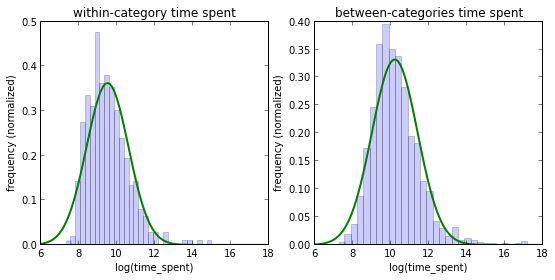
\includegraphics[width=0.9\columnwidth]{hyp5_comparison}
    \caption{Time spent to generate an instance}
    \label{fig:hyp5_comparison}
\end{figure}

The resulting models fitted to the data are shown in Figure~\ref{fig:hyp5_comparison}. The mean for the within-category condition was 9.5 in log space (13.4 seconds, HDI 9.4-9.6), while the mean for the between-categories condition was 10.2 (27.0 seconds, HDI 10.2-10.3). The differences in mean are significant and confirm hypothesis 5. Notably, within-category instance generation took an average of 12.6 seconds less than between-categories instance generation, consistent with the findings of Nijstad and Stoebe, who reported differences of 6-12 seconds between these two idea generation processes.

%Figure FIG displays the mean time spent on an instance by order, separated by condition. Most of the highly variant response times take place early in the brainstorming run. This suggests that at least one participant accepted a brainstorming task, took an initial stab at instances, and then left the task for up to 8 hours before continuing. Beyond this, we might expect to see time spent per instance go up as participants have to dig deeper to find responses, but no such effect is consistently observed.

% \begin{figure}[h]
%     \centering
%     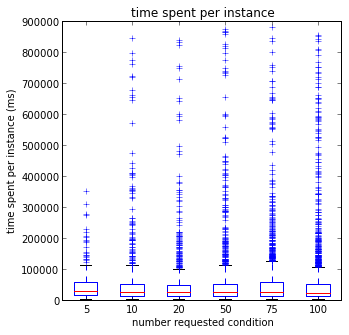
\includegraphics[width=0.9\columnwidth]{time_spent_condition}
%     \caption{Time spent per instance}
% \end{figure}


% \begin{figure}[h]
%     \centering
%     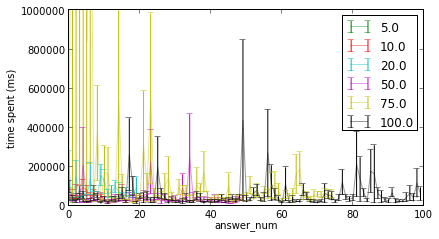
\includegraphics[width=0.9\columnwidth]{time_spent_order}
%     \caption{Time spent per instance}
% \end{figure}


%The Nijstad and Stroede \cite{nijstad_how_2006} model also provides \textbf{Hypothesis 5}: \emph{idea generation when changing semantic categories should take longer than idea generation within categories}. 

